\documentclass{article}
\usepackage{tikz}
\usetikzlibrary{arrows.meta}

\begin{document}

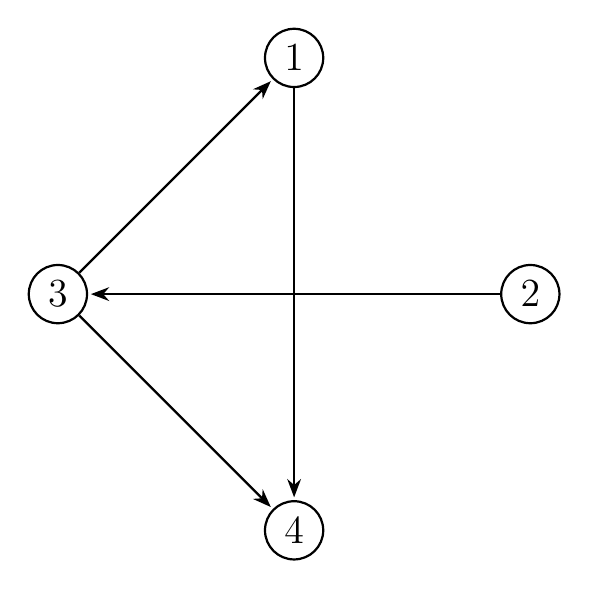
\begin{tikzpicture}[->,>=Stealth,shorten >=1pt,auto,node distance=3cm, thick,main node/.style={circle,draw,font=\sffamily\Large\bfseries}]
\node[main node] (2) at (3.00,0.00) {$ 2 $};
\node[main node] (1) at (0.00,3.00) {$ 1 $};
\node[main node] (3) at (-3.00,0.00) {$ 3 $};
\node[main node] (4) at (-0.00,-3.00) {$ 4 $};
\path (1) edge  (4);
\path (2) edge  (3);
\path (3) edge  (1);
\path (3) edge  (4);
\end{tikzpicture}

\end{document}